\documentclass[acmtallip]{acmsmall} % Aptara syntax  %  prodmode,

\usepackage[ruled]{algorithm2e} % For algorithms
\renewcommand{\algorithmcfname}{ALGORITHM}
\SetAlFnt{\small}
\SetAlCapFnt{\small}
\SetAlCapNameFnt{\small}
\SetAlCapHSkip{0pt}
\IncMargin{-\parindent}


\usepackage{CJKutf8}
\usepackage{graphicx}
\usepackage{url}
\usepackage{subfigure}
\usepackage{latexsym}
\usepackage{multirow}
\usepackage{footnote}
\usepackage{array}
\usepackage{amsmath}
\usepackage{bm}
\usepackage{booktabs}
\usepackage{threeparttable}


\usepackage{color, colortbl}

\definecolor{Gray}{gray}{0.9}




\renewcommand{\algorithmcfname}{ALGORITHM}
\SetAlFnt{\small}
\SetAlCapFnt{\small}
\SetAlCapNameFnt{\small}
\SetAlCapHSkip{0pt}
\IncMargin{-\parindent}

% Metadata Information
%\acmVolume{9}
%\acmNumber{4}
%\acmArticle{39}
%\acmYear{2010}
%\acmMonth{3}
\DeclareMathOperator*{\argmax}{\arg\!\max}
\DeclareMathOperator*{\logadd}{\log\!\mathrm{add}}

% New Commands
\newcommand\FIXME[1]{\textcolor{red}{FIX:}\textcolor{red}{#1}}
\newcommand{\CBiLSTM}{\texttt{C-BiLSTM}\xspace}
\newcommand{\BiLSTM}{\texttt{BiLSTM}\xspace}
\newcommand{\CNN}{\texttt{CNN}\xspace}
\newcommand{\CBiLSTMCRF}{\texttt{C-BiLSTM-CRF}\xspace}
\newcommand{\CRF}{\texttt{CRF}\xspace}
\newcommand{\LSTM}{\texttt{LSTM}\xspace}
\newcommand{\SRL}{\texttt{SRL}\xspace}
\newcommand{\NER}{\texttt{NER}\xspace}
\newcommand{\POS}{\texttt{POS}\xspace}


% DOI
\doi{0000001.0000001}

%ISSN
\issn{1234-56789}

% Document starts
\begin{document}

% Page heads
\markboth{Y. Zeng et al.}{Neural Chinese Event Extraction}

% Title portion
\title{Neural Chinese Event Extraction}
\author{
YING ZENG
\affil{Peking University}
YANSONG FENG
\affil{Peking University}
HONGHUI YANG
\affil{Peking University}
ZHENG WANG
\affil{Lancaster University}
DONGYAN ZHAO
\affil{Peking University}
}

\begin{abstract}
Event extraction is an important technology that underpins many text mining applications. It is a task of extracting events of
certain types and their corresponding arguments of different roles from unstructured texts such as news articles and tweets.
State-of-the-art event extraction approaches rely on high quality feature extraction that requires careful template design
and is dependent on the results of specific semantic or lexical analyzing tools as well as extra thesauruses.
As a result, current approaches are hard to generalize, and are not portable to new languages, especially those with limited resources or tools.


Different from English, the unique language structures and syntax of Chinese make  prior work on English event
extraction inapplicable to the new domain.  In this work, we demonstrate that, for the first time, it is possible to
construct a generalized yet effective Chinese event extraction model without relying on manually designed feature
templates or specific lexical or syntactic tools. Our novel, broadly applicable approach employs a convolution
bidirectional long short-term memory neural network (\CBiLSTM) to automatically learn a set of effective feature
representations. We achieve this by exploiting different neural network components to extract features at various
levels. More specifically, we employ  a convolutional component (\CNN) for prominent lexical features and a
bidirectional long short-term memory component (\BiLSTM) for capturing sentence level representations. To overcome the
language-specific challenge of Chinese word segmentation, we combine a conditional random field (\CRF) layer over a
character-level neural network component to allow us tag each character beyond the word boundary. We evaluate our
approach by applying it to the ACE 2005 dataset. The experimental results show that our approach can deliver
state-of-the-art performance in both trigger labeling and argument labeling without laborious feature engineering.



%In this paper, we
%propose a convolution bidirectional long short-term memory neural network (C-BiLSTM)  model that benefits different
%neural network components to learn both lexical and sentence level feature representations without relying on manually
%designed feature templates or complicated lexical or syntactic tools.  We further propose to combine a CRF layer over a
%character-level neural network components to address the language specific issues in Chinese event extraction.
%Experiments on ACE 2005 dataset show that our approaches can achieve state-of-art performances in both trigger labeling and
%argument role labeling, without feature engineering or extra resources.
\end{abstract}


\begin{CCSXML}
<ccs2012>
<concept>
<concept_id>10010147.10010178.10010179.10003352</concept_id>
<concept_desc>Computing methodologies~Information extraction</concept_desc>
<concept_significance>500</concept_significance>
</concept>
</ccs2012>
<ccs2012>
<concept>
<concept_id>10010147.10010178.10010179.10003352</concept_id>
<concept_desc>Computing methodologies~Information extraction</concept_desc>
<concept_significance>500</concept_significance>
</concept>
<concept>
<concept_id>10010147.10010257.10010293.10010294</concept_id>
<concept_desc>Computing methodologies~Neural networks</concept_desc>
<concept_significance>500</concept_significance>
</concept>
</ccs2012>
\end{CCSXML}

\ccsdesc[500]{Computing methodologies~Information extraction}
\ccsdesc[500]{Computing methodologies~Neural networks}




% We no longer use \terms command
%\terms{Design, Algorithms, Performance}

\keywords{Event Extraction, Chinese Natural Language Processing, Neural Network Models}

% At a minimum you need to supply the author names, year and a title.
% IMPORTANT:
% Full first names whenever they are known, surname last, followed by a period.
% In the case of two authors, 'and' is placed between them.
% In the case of three or more authors, the serial comma is used, that is, all author names
% except the last one but including the penultimate author's name are followed by a comma,
% and then 'and' is placed before the final author's name.
% If only first and middle initials are known, then each initial
% is followed by a period and they are separated by a space.
% The remaining information (journal title, volume, article number, date, etc.) is 'auto-generated'.

\acmformat{Ying Zeng, Yansong Feng, Honghui Yang, Zheng Wang, Dongyan Zhao, 2017. Neural Chinese Event Extraction}


\begin{bottomstuff}
\emph{Extension of Conference Paper:} a preliminary version of this article entitled ``A convolution BiLSTM neural
network model for Chinese event extraction" by Y. Zeng, Y. S. Feng, H. H. Yang, Z. Wang and D. Y. Zhao appeared in the 24th
International Conference on Computer Processing of Oriental Languages, ICCPOL 2016 \FIXME{\cite{}}. The extended
version makes the following new contributions over the conference paper: \FIXME{(1) it provides xxx
(Section xx); (2) it describes the selection xx (Section xx); (3) it provides new experimental results xxx (Section
xx)...}


This work was partially supported by the National High Technology R\&D Program of China under Grant No. 2015AA015403,
  the Natural Science Foundation of China under Grant agreements 61202233, 61272344 and 61370055, the UK Engineering
  and Physical Sciences Research Council under grants EP/M01567X/1 (SANDeRs) and EP/M015793/1(DIVIDEND), and a joint
  project with IBM Research. Any correspondence please refer to Yansong Feng.

Author's addresses: Y. Zeng {and} Y. Feng {and} H. Yang {and} D. Zhao, Institute of Computer Science and Technology,
    Peking University, P.R. China; Z. Wang, School of Computing and Communications, Lancaster University, UK.
\end{bottomstuff}


% The default list of authors is too long for headers}
%\renewcommand{\shortauthors}{Y. Zeng et al.}

\maketitle

\begin{CJK}{UTF8}{gbsn}

\section{Introduction}

Event extraction is the task of finding specific events and then extracting structured knowledge of the events from
unstructured data such as news articles, tweets, or blogs. It is an important technique that underpins many text mining
applications such as news recommendation and information filtering.
The goal of event extraction is to discover structured information about an event occurrence like ``\emph{who did what to whom,
when, where through what methods, and why}"~\cite{Piskorski2013}. A concrete example of event extraction is
given in Figure 1. Given a text
document, an event extraction system should be able to identify all the relevant entities and their relationships.

Finding a set of high-quality features, i.e. feature engineering, is key to event extraction.
Most current approaches rely on hand-crafted features to build multi-class classifiers to perform various
event-extraction-related tasks~\cite{ahn2006stages,chen2009language,li2012employing,chen2012joint}. The
features used in prior work can be divided into two categories: \emph{lexical features} and \emph{sentence-level features}, where the
former are designed to capture the local information of words, such as part-of-speech tags or word lemma, while the latter are used to
characterize the topic of the whole sentence. The challenge of finding useful
features is that the space of possible features is vast, while their effect depends on various factors: the natural language, the structure of the data, and the application domain.

Despite much progress has been made in English event extraction, building an effective Chinese event extraction system
remains a challenge. There have been efforts to solve this problem using hand-crafted feature templates
building upon specific natural language processing (NLP) tools, such as POS tagging~\cite{}, syntactic parsing~\cite{}, semantic role labeling~\cite{}, and so on.
While it is possible to manually design a set of task-specific feature templates, current approaches require extensive human involvement
and are tightly couple to the information provided by specific NLP tools. This means that when we target a new  language,  where limited tools or resources are available,
despite of the time-consuming process of feature engineering, the system will be heavily affected by the performance of existing NLP tools
for that new language. Unfortunately, most low-resourced languages have far-from-perfect performances even in their fundamental semantic or
syntactic analysis, e.g., Chinese syntactic parsing performance is around 5\% lower than that of English in newswire, which leads to significant
performance drop in downstream applications.
%However,  manually performing this costly feature-tuning process for each individual domain or NLP tool is
%unrealistic due to the drastic effort involved. Given the fast evolving natural of software tools and application domains,
Therefore, it is essential to have a technique that can automatically discover lexical and sentence-level
feature representations for event extraction in a low-resourced language, without extensive human involvement and the heavy reliance on specific NLP tools.

In this paper, we propose to utilize neural networks to alleviate the burden of feature
engineering for Chinese event extraction. To do so, we develop a convolution bidirectional long short-term memory
(\LSTM) network (\CBiLSTM) to automatically learn lexical and sentence level feature representations without extensive human
involvement. We achieve this by first constructing a bidirectional \LSTM to encode the entire sentence into
sentence-level features without performing dependency parsing or semantic role labeling (\SRL). % -- which require inputs from human experts~\cite{}.
We then take advantage of a convolutional neural network to capture salient local features
to semantically characterize event occurrences, %recognize and classify how the event is triggered,
without relying on part-of-speech (\POS) tagging or named entity
recognition (\NER). %This allows us to build a system to automatically extract local lexical features.
To address the word segmentation issue, a fundamental yet challenging step for Chinese language processing, we employ
a conditional random field (\CRF) layer to automatically learn sentence-level labeling constraints and jointly decode
the best labeling sequence for the whole sentence.

Putting together these techniques, we are able to build a powerful
system for Chinese event extraction. As we show, our approach can
automatically learn feature representations that lead to the same level of performance compared to hand-tuned features selected by %independent
human experts. This is truly remarkable when one considers that our approach is given no prior knowledge of
the syntax or semantics of the target language. %\FIXME{Check the last sentence.}

We evaluate our approach on the ACE 2005 Chinese event extraction corpus which consists of 8 event types and 33 subtypes.
We compare our approach against a set of well-established traditional feature-based models available for this heavily-studied data set.
The experimental results show that our automatic approach can effectively learn both local semantic and sentence level
representations for event extraction and deliver state-of-the-art performance, when compared to
the hand-tuned features developed by human experts.

%The technical contributions of this work can be summarized as follows. It is the first to
%\begin{itemize}
%\item blabla
%\item blabla
%\item blabla
%\end{itemize}

The rest of this paper is organized as follows. Section~\ref{background} explains the terminologies and defines the
scope of the work. Section~\ref{related} discusses related Chinese event extraction systems. Section ~\ref{trigger} and
Section~\ref{argument} present the neural network models applied to trigger labeling and argument labeling.
Section~\ref{experiment} presents the experimental results and analyses. We conclude our work in
Section~\ref{conclude}.

\section{Background and Problem Definition}
\label{background}
%\subsection{Terminologies}
This work focuses on the
event extraction task proposed by the Automatic Content Extraction (ACE) program \cite{doddington2004automatic} which
defines the following terminologies for event extraction:

\begin{itemize}
	\item \textbf{Event mention}:  a phrase or sentence within which an event is described, including a trigger and its arguments.
	\item \textbf{Event trigger}: the main word or phrase that most clearly expresses the occurrence of an event. An event trigger is typically a verb or a noun in the ACE framework.
	\item \textbf{Event argument}: an entity, temporal expression or value that is involved in an event.
	\item \textbf{Argument role}: the relationship between an argument and the event in which it participates.
\end{itemize}

Specifically, in the initial 2005 evaluation, there are three languages in the ACE event extraction task,  English, Chinese and Arabic. Similar to many other NLP tasks, English event extraction receives relatively more attention in the literature, while Chinese and Arabic are not in the spotlight.  In this paper, we aim to improve Chinese event extraction.

Despite of the differences among these three languages, their ACE task setups remain the same.
Given a text document, an event extraction system need to identify all event triggers with specific types and their corresponding arguments for each sentence. For example, given an example sentence, S1, in Chinese, the system should produce a structured output, including a typed event trigger  and its corresponding arguments  with pre-defined  roles, as shown in Figure~\ref{exfigure}.

\begin{figure}
\centering
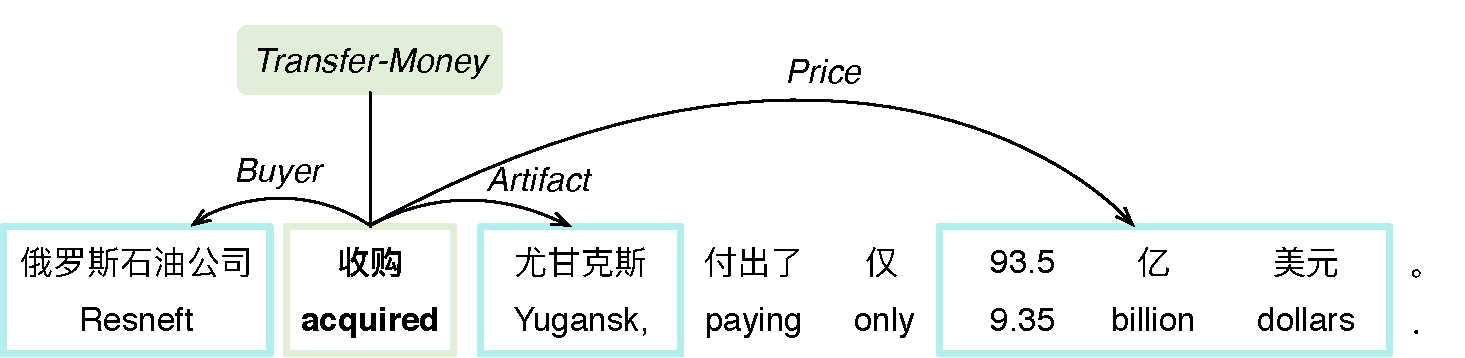
\includegraphics[width=.9\textwidth]{example.pdf}
\caption{An example of Chinese event extraction for S1, where English translations are provided besides the Chinese words. The example sentence has one \emph{Transfer-Money} event mention triggered by \textit{收购 (acquired)}, which have three arguments, \textit{俄罗斯石油公司 (Rosneft)} as the \emph{Transfer-Money} event's \textit{Buyer}, \textit{尤甘斯克 (Yugansk)}  as its \textit{Artifact}, and \textit{93.5 亿美元 (9.35 billion dollars)} as its \textit{Price}.}
\label{exfigure}
\end{figure}

\begin{quote}
S1: 俄罗斯石油公司 \hspace{0.3cm}收购 \hspace{0.3cm}尤甘斯克 \hspace{0.3cm}付出 \hspace{0.2cm}了 \hspace{0.2cm}仅 \hspace{0.3cm}93.5 \hspace{0.3cm}亿 \hspace{0.3cm}美元。

\hspace{0.52cm} Rosneft acquired Yugansk, paying only 9.35 billion dollars.
\end{quote}

To produce such a structured output, a system usually has to solve the following four subtasks,
\begin{enumerate}
	\item \textbf{Trigger identification}: recognize the event trigger from the sentence, e.g., \textit{``收购'' (acquired)} should be identified as a trigger of an event;
	\item \textbf{Trigger classification}: assign an event type for the identified trigger, e.g., \textit{``收购'' (acquired)} should be assigned with the type \emph{Transfer-Money};
	\item \textbf{Argument identification}: determine whether a word or phrase plays a certain role in the event mention, e.g., \textit{``俄罗斯石油公司'' (Rosneft)}, \textit{``尤甘斯克'' (Yugansk)}, and \textit{``93.5亿美元'' (9.35 billion dollars)} are the arguments of this \emph{Transfer-Money} event;
	\item \textbf{Argument classification}: assign a role to each identified argument, e.g., \textit{``俄罗斯石油公司'' (Rosneft)}, \textit{``尤甘斯克'' (Yugansk)}, and \textit{``93.5亿美元'' (9.35 billion dollars)} play the roles of \emph{Buyer}, \emph{Artifact} and \emph{Price}, respectively, in this  \emph{Transfer-Money} event.
\end{enumerate}


However, such a 4-step pipeline system inevitably suffers from the error propagation problems, let alone language specific challenges,  e.g., Chinese word segmentation, and insufficient capability of existing NLP tools for those low-resourced languages.  As addressed in the literature \cite{chen2009language,li2012employing}, errors made by an upstream subtask, e.g., Chinese word segmentation or trigger identification,  will propagate to the downstream subtasks, e.g., tigger classification or argument identification, and could adversely affect their performance. In most cases, downstream subtasks will have no chance to even alleviate such effect. The work presented in \cite{chen2012joint} addresses the issue by recasting the 4-step framework  into two joint learning tasks, namely, \textbf{trigger labeling} and \textbf{argument labeling}. The  former jointly learns trigger identification and classification, while the latter learns argument identification and argument classification simultaneously, which has been shown to be promising in Chinese event extraction~\cite{chen2012joint}. In this work, we follow this 2-step approach for Chinese event extraction.


Previous state-of-the-art approaches in Chinese event extraction~\cite{chen2009language,li2012employing,chen2012joint,li2013joint} usually rely on a variety of elaborate features, which, in general, must be designed by experts, and extracted using lexical or syntactic analysis tools. Those features can be roughly divided into two categories: \textbf{lexical features} and \textbf{sentence-level features}. The former are designed to capture local features, while the latter characterize global topics of the sentences.  Take trigger labeling in the following sentences as an example: the target word \textit{``成立'' (found)} indicates a \emph{Business} event in S2, but not in either S3 or S4.

\begin{quote}
S2: Intel 在 中国 \textbf{成立} 了 研究中心。

\hspace{0.52cm} Intel \textbf{founds} a research center in China.
\end{quote}

\begin{quote}
S3: 它 \textbf{成立} 于 1994 年 , 现在 是 一支 深 受 欢迎 的 乐队。

\hspace{0.52cm} It was \textbf{founded} in 1994, and now is a very popular band.
\end{quote}

\begin{quote}
S4: 医院 已 \textbf{成立} 救援中心。

\hspace{0.52cm} The hospital has \textbf{founded} rescue centers.
\end{quote}

\textbf{Lexical features}, often in the form of word lemma or part-of-speech tags (POS), provide semantic information of a candidate word and its surrounding context. In S4, the neighboring word ``救援中心''(rescue center) serves as a lexical feature for \textit{``成立'' (found)}, indicating a medical institute,  thus we can infer that \textit{``成立'' (found)} is not a trigger of a \emph{Business} event.

\textbf{Sentence-level features} are usually extracted from syntactic structures, and  maintain important clues about the whole sentence. S3 talks about ``它\_是\_乐队'' (it\_is\_band) and ``它\_成立\_1994'' (it\_founded\_1994), indicating the verb ``成立'' (founded) relates to a musical group, thus should not be regarded as a trigger of a \emph{Business} event.

%\subsection{Problem Scope}
The aim of this work is to investigate ways to automatically find effective features for \textbf{trigger labeling} and \textbf{argument labeling}.
Although event extraction (mainly argument labeling) also depends on name identification and entity mention co-reference, which are challenging by themselves, these techniques fall out of the scope of this work. In comply with the standard practice in prior work~\cite{chen2009language,chen2012joint}, we directly utilize the entity recognition ground-truth provided by ACE for argument labeling. We stress that other work on improving argument labeling is thus orthogonal to our approach.

%\subsection{Drawbacks of Manual Feature Engineering}
Traditional event extraction methods \cite{ahn2006stages,chen2009language,li2012employing,chen2012joint} rely on those carefully-designed features to build multi-class classifiers for each subtask. They first apply a series of NLP tools to extract lexical features (e.g., \POS tagging, and named entity recognition (\NER)) and sentence-level features (e.g., dependency parsing, and semantic role labeling (\SRL)). Then in the training stage, they learn to weight each feature for each subtask in the pipeline, independently, with a classifiers, e.g., conditional random fields (\CRF) \cite{lafferty2001conditional}, support vector machines~\cite{suykens1999least}, maximum entropy \cite{phillips2006maximum}, etc. Although those methods can achieve satisfactory performances, they still suffer from the hard feature engineering, where human expert involvement is necessary,  and many semantic/syntactic tools may not work as well as we expected. This is a particular problem for low-resourced languages, for which the overall performance is often below 70\%, resulting in incorrect feature extraction and confusing the classifier.

\begin{quote}
	S5: 犯罪 嫌疑人 都 \textbf{落入 法网}。
	
	\hspace{0.55cm} The suspects were \textbf{arrested}.
\end{quote}
\begin{quote}
	S6: 警察 \textbf{击毙} 了 一名 歹徒。
	
	\hspace{0.55cm} Polices \textbf{shoot} and \textbf{kill} a criminal.
\end{quote}
\begin{quote}
	S7: 这 是 一件 预谋 的 \textbf{凶杀}案。
	
	\hspace{0.55cm} It is a premeditated \textbf{murder} case.
\end{quote}

Take Chinese event extraction systems as an example. Current Chinese systems do not perform as well as their English counterparts. One of the major obstacles, as suggested by \citeN{li2012employing}, is caused by the Chinese word segmentation, a unique preprocessing step for Chinese. Unlike English, Chinese does not have delimiters between words, which makes word segmentation the very first and fundamental step in Chinese event detection. However, we find that word segmentation granularity does have a great impact on the trigger labeling performance. For example, triggers in S5$\sim$S7 cannot be recognized accurately if we simply predict whether a word is an event trigger or not. In S5, the word ``落入法网'' is usually separated into two words, while the gold-standard trigger is ``落入法网'' as a whole; while in S6, ``击毙'', in most cases, is treated as one single word, but actually, the characters ``击'' and ``毙'' are two triggers of different types, the former an \textit{Attack} event and the latter a \textit{Die} event, respectively. As in such a pipeline framework, incorrect trigger labeling will definitely affect downstream argument labeling, whose inputs are highly related to the predicated triggers.

One of the key innovations of our approach is to recast trigger labeling as a sequence labeling task, and further to combine different neural network components to automatically learn feature representations of different levels capturing both local lexical and sentence level characteristics for event extraction. Doing so allows us to  address the Chinese language-specific issues mentioned above, by exploiting the recent breakthrough effectiveness of deep neural networks in natural language modeling, and to alleviate the burden of hard feature engineering and the reliance on external tools or thesauruses. In the reminder of this paper, we will describe how to build such a system in two-step fashion, trigger labeling and argument labeling.


\section{Trigger Labeling}\label{trigger}
Trigger labeling, also called event detection, aims to discover event triggers and assign them a predefined event type. We jointly learn trigger identification and type classification by one network to reduce the error propagation problem in a pipeline model. Before we present our solution, we first discuss the language specific issues in Chinese trigger labeling.

\subsection{Language Specific Issues}
We summarize the inconsistency problems between words and triggers as the following two types.

\begin{enumerate}
	\item Cross-word triggers: While many events anchor on a single word, multiple words could reasonably be called a trigger. In S4, the \emph{arrest\_jail} event should be triggered by neither ``落入'' nor ``法网'', but ``落入法网'' (arrested).
	\item Inside-word triggers: Almost all Chinese characters have their own meanings, and some of which can be triggers themselves. There may be greater than one trigger in a word like ``击毙'' (shoot and kill). Continuous characters of a word can also form a trigger such as ``凶杀'' (murder) in ``凶杀案'' (murder case).
\end{enumerate}

Table~\ref{tab:one} summarizes the number of problematic triggers we found in ACE 2005 Chinese corpus using different Chinese word segmentation tools. Even the minimum inconsistency rate is as high as 14\%.

\begin{savenotes}
\begin{table}
\centering
\tbl{Numbers of triggers inconsistent with the words.\label{tab:one}}{
\begin{tabular}{|l|c|c|c|} \hline 
NLP Tool & Cross-word Trigger & Inside-word Trigger & Total \\ \hline
Stanford NLP\footnote{\texttt{http://nlp.stanford.edu/software/segmenter.shtml}} & 14.6\% & 5.0\% & 19.6\% \\ \hline
Jieba\footnote{\texttt{https://github.com/fxsjy/jieba}} & 16.6\% & 2.6\% & 19.2\% \\ \hline
NLPIR\footnote{\texttt{https://github.com/NLPIR-team/NLPIR}} & 8.9\% & 5.2\% & 14.1\% \\ \hline
\end{tabular}}
\end{table}
\end{savenotes}

To address the language specific issues, we treat event detection as a sequence labeling task. Formally, we use $\bm{w}=\{w_1, w_2, \ldots, w_n\}$ to represent an input sentence of length $n$, where $w_i$ is the $i$-th word. And $\bm{y}=\{y_1, y_2, \ldots, y_n\}$ represents a generic sequence of labels for $\bm{w}$. Each word is tagged in the \texttt{BIO} scheme, where each token is labeled as \texttt{B-type} if it is the beginning of an event trigger with event type \texttt{type}, or \texttt{I-type} if it is inside a trigger, or \texttt{O} otherwise. Our first labeling model is a word-based bidirectional LSTM network (BiLSTM) with a CNN layer as shown in Figure~\ref{fig:1}.

\subsection{Word-based Convolution BiLSTM Model \label{wcblstm}}
In this section, we introduce the components (layers) in our Convolution BiLSTM (C-BiLSTM) network one-by-one from bottom to top.
\begin{figure}
\centering
\subfigure[Convolution BiLSTM network]{\label{fig:a}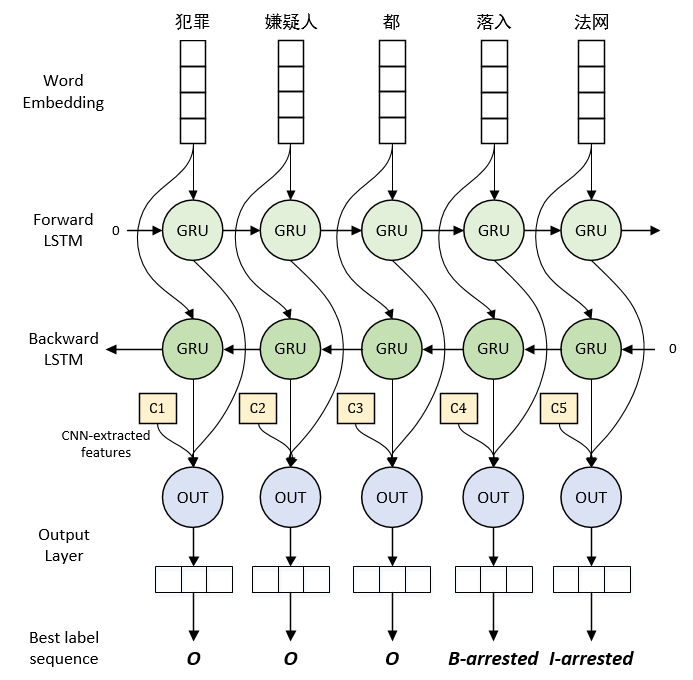
\includegraphics[width=0.62\textwidth]{RNN1.png}}
\subfigure[Details of CNN in (a)]{\label{fig:b}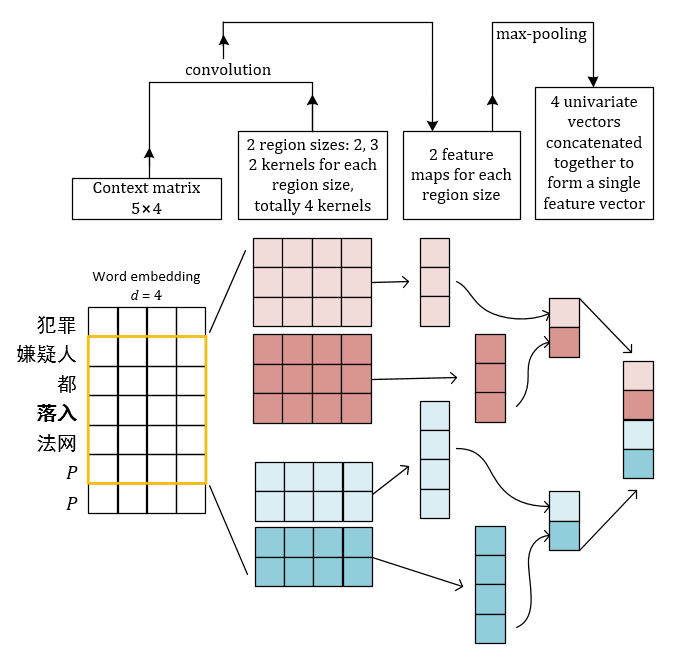
\includegraphics[width=0.62\textwidth]{CNN1.png}}

\caption{The main architecture of our word-based convolution bidirectional LSTM model. The local contextual feature $c_{i}$ (yellow rectangle) in (a) for each word $w_i$ is computed by the CNN as (b) illustrated. Our CNN layer learns a representation of local context information about the center word ``落入''. Here the context size is 5 (2 words to the left and to the right of a center word), and we depict two kernel region sizes: 2 and 3, each of which has 2 kernels. The symbol \emph{P} in sentence of (b) represents a padding word.\label{fig:1}}

\end{figure}

\paragraph{LSTM Network}
Recurrent neural networks (RNNs) maintain a memory based on historical contextual information, which makes them a natural choice for processing sequential data. Unfortunately, it is difficult for standard RNNs to capture long range dependencies due to vanishing/exploding gradients \cite{bengio1994learning}. Long Short-Term Memory Network \cite{hochreiter1997long} is explicitly designed to solve the long-term dependency problem through purpose-built memory cells. They consist of several multiplicative gates that control the proportion of information to forget and to store in the cell states. In this paper, we apply a variation of LSTM units, Gated Recurrent Unit (GRU) \cite{cho2014learning}, which is found to be superior to LSTM on a suit of tasks by Chung et al. \shortcite{chung2014empirical}. The GRU is implemented as the following formulas:
\begin{align*}
	\text{r}_t &= \sigma(\text{W}_{xr}\text{x}_t + \text{W}_{hr}\text{h}_{t-1} + \text{b}_r) \\
	\text{z}_t &= \sigma(\text{W}_{xz}\text{x}_t + \text{W}_{hz}\text{h}_{t-1} + \text{b}_z) \\
	\tilde{\text{h}}_t &= \tanh(\text{W}_{xh}\text{x}_t + \text{W}_{hh}(\text{r}_t \odot \text{h}_{t-1}) + \text{b}_h) \\
	\text{h}_t &= \text{z}_t \odot \text{h}_{t-1} + (1 - \text{z}_t) \odot \tilde{\text{h}}_t
\end{align*}

In these formulas, the $\text{W}_*$ variables are the weight matrices and the $\text{b}_*$ variables  are the biases. $\sigma(\cdot)$ is the element-wise sigmoid function and $\odot$ is the element-wise product.

Formally, we use $\text{x}_t$ to represent the feature vector (e.g. word embedding) corresponding to the $t$-th word $w_t$. At each time step $t$, a GRU takes $\text{x}_t$ as input and computes the hidden state (also called output vector) $\text{h}_t$ by reset gate and update gate. The reset gate $\text{r}_t$ controls how much and what information from the previous hidden state should be reset, and the update gate $\text{z}_t$ determines how much the unit updates its previous hidden state.

\paragraph{BiLSTM Network}
In the event extraction task, if we can access to both past and future contexts for a candidate trigger, we can explore richer sentence-level information and make better prediction. This can be done by bidirectional LSTM networks \cite{graves2005framewise,graves2013speech}. Figure 1(a) shows the layers of a BiLSTM trigger identification model.

At time $t$, a forward LSTM network computes the hidden state $\overrightarrow{\text{h}_t}$ of the past (left) context of the sentence at word $w_t$, while a backward LSTM network reads the same sentence in reverse and outputs $\overleftarrow{\text{h}_t}$ given the future (right) context. We concatenate these two vectors to form the output vector of a BiLSTM network, i.e. $\text{B}_t = [\overrightarrow{\text{h}_t}; \overleftarrow{\text{h}_t}]$.

\paragraph{CNN Layer}
Convolutional neural networks (CNNs) are originally applied to computer vision to capture salient local features \cite{lecun1998gradient}. Previous studies on event extraction \cite{nguyen2015event,chen2015event,feng2016language} have gradually shown that CNN architectures are effective to capture semantic features similar to n-grams, but represent them in a more compact way. We employ a convolutional neural network as illustrated in Figure 1(b) to extract local contextual information for each word in a sentence.
Specifically, for every word in the sentence, we want to extract local contextual information to help predict whether the current word is an event trigger. The current word $w_i$ along with its context constitutes the input of CNN. Let $w_{i:i+j}$ be the window of words from $w_i$ to $w_{i+j}$, and $2k+1$ be the fixed context size. So the context window $c_i$ (padded when necessary) where the current word $w_i$ is in the middle can be written as
\begin{equation}
	c_i = w_{i-k:i+k} = [w_{i-k}, \ldots, w_{i}, \ldots, w_{i+k}].
\end{equation}
Before being fed into a convolution layer, each word $w_i$ is transformed into a d-dimensional word vector $\text{x}_i$ by looking up the embedding table. As a result, the original context $c_i$ is transformed into a matrix $\bm{c}_i = [\text{x}_{i-k}, \ldots, \text{x}_i, \ldots, \text{x}_{x+k}]$ of size $(2k+1) \times d$. The matrices $\bm{c}_1$, \ldots, $\bm{c}_n$ are then passed through a convolution layer and a max pooling layer.
In the convolution layer, we utilize a set of kernels $\{\text{w}_1, \text{w}_2, \ldots, \text{w}_m\}$ with various widths to extract semantic features like n-grams of different granularities. For every context matrix $\bm{c}_i$, a kernel $\text{w}_j$ of width $l$ is applied to all possible windows of $l$ words within the context (i.e., $w_{i-k:i-k+l-1}$, \ldots, $w_{i+k-l+1:i+k}$). And $\text{w}_j$ can be essentially seen as a weight matrix of size $l \times d$. For example, the convolution operation involves kernel $\text{w}_j$ over the window $w_{t:t+l-1}$ can be express as:
\begin{equation} s_{jt}=f(\text{w}_j \cdot \text{x}_{t:t+l-1} + b_j), 1 \leq j \leq m, i-k \leq t \leq i+k-l+1 \end{equation}
where $b$ is a bias term and $f$ is a non-linear function such as hyperbolic tangent. The convolution result is a feature map $\text{s}_j \in \mathbb{R}^{2k-l+2}$.
We then perform a max-over-time pooling operation \cite{collobert2011natural} over each feature map,
\begin{equation}
\tilde{s}_j=\max\{\text{s}_j\}=\max\{s_{j1}, s_{j2}, \ldots, s_{jm}\}	
\end{equation}
so that only the largest number is recorded. One property of pooling is that it produces a fixed size output vector, which enables us to apply variable kernel sizes. And by performing the max operation, we are keeping the most salient information. Finally, we take the fixed length output vector $\text{C}=[\tilde{s}_1, \tilde{s}_2, \ldots, \tilde{s}_m]$ as a representation of local contextual information about the current word.

In our implementation, the context window size is 7 (3 words to the left and to the right of a center word), and kernel sizes from 2 to 7 to encode the semantics of n-grams with various granularities. Each kernel generates 32 feature maps.

\paragraph{Output Layer\label{output}}
For each word $w_i$ in the sentence, we concatenate the bidirectional sentence-level features $\text{B}_i$ learned by BiLSTM, and the contextual semantic features $\text{C}_i$ extracted by CNN, into a single vector $\text{F}_i=[\text{B}_i;\text{C}_i]$. To compute the confidence of each label, the final feature vector $\text{F}_i \in \mathbb{R}^{2d_{gru}+d_{cnn}}$, where $d_{gru}$ is the dimension of the GRU unit and $d_{cnn}$ is the number of feature maps in CNN layer, is fed into a fully connected linear layer.
\begin{equation}
	 \text{O}_i = \text{W}_s\text{F}_i+\text{b}_s
\end{equation}

where $\text{W}_s \in \mathbb{R}^{n_{e} \times (2d_{gru} + d_{cnn})}$ is the transformation matrix and $\text{O}_i=[O_{i,1}, \ldots, O_{i,{n_e}}]$ is the final output vector, $n_{e}$ is the number of distinct labels, and the $e$-th element $O_{i, e}$ indicates the score for label $e$.

Then $\text{O}_i \in \mathbb{R}^{n_e}$ is fed into a softmax layer to estimate a probability distribution over all possible labels. In the end, we choose the label that obtains maximum probability as the prediction for $y_i$.
\begin{equation}
	P(e \mid \text{O}_i) = \frac{\exp{(O_{i,e})}}{\sum\nolimits_{j=1}^{n_e}\exp{(O_{i,j})}}
\end{equation}
\begin{equation}
  	y_i = \argmax\limits_{e}{P(e \mid \text{O}_i)}
\end{equation}

\paragraph{Errata Table}
However, this word-base model still suffer from  the inconsistency problem caused by inside-word triggers. Inspired by \citeN{chen2009language}, we construct a global errata table to record some frequent appearances of tokens and triggers in the training set. In our experiments, if 80\% occurrences of a token inside a word should be labeled as triggers with the same event type, we then add this ``word$-$token$-$type'' triple into the table. During testing, if a word has an entry in the errata table, we regard its token as a trigger with the event type according to the corresponding triple directly. For example, if ``击毙$-$击$-$\emph{Attack}'' and ``击毙$-$毙$-$\emph{Die}'' are two triples in the errata table, word-based C-BiLSTM model can identify all inside-word triggers in S6 correctly.

\subsection{Character-based Convolution BiLSTM Model \label{ccblstm}}
\begin{figure}
\centering
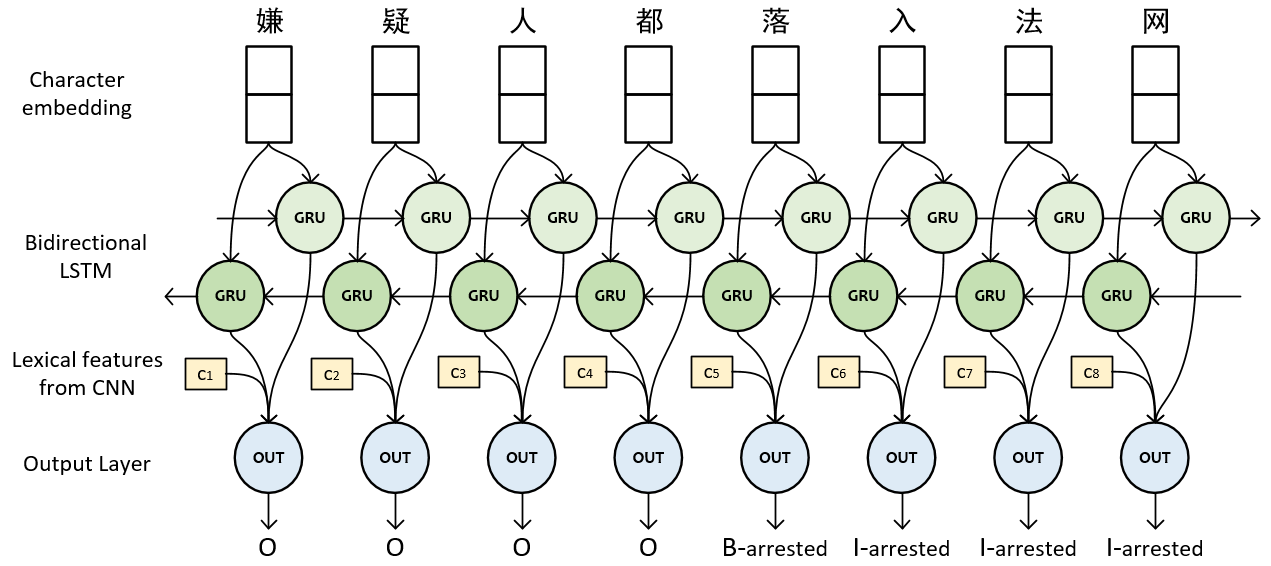
\includegraphics[width=.9\textwidth]{RNN2.png}
\caption{Character-based Convolution BiLSTM network.}
\label{figure2}
\end{figure}

Despite of the effectiveness of errata table, word-based method is not a perfect solution to language specific issues, because it only recognizes triggers in a word level or frequent inside-word triggers appearing in training data. When it comes to an unknown inside-word trigger which never occurs during training, there is no way for an errata table to label it correctly.

Ideally, character-based methods may solve both inconsistency problems, which use the same \texttt{\{BIO\}-type} tagging scheme as word-based model, however, to label each character rather than each word. For better understanding, resulting sequences of example sentences S4 and S5 labeled by two models are listed in Table~\ref{six}.

As shown in Figure~\ref{figure2}, character-based C-BiLSTM has a similar network architecture as word-based C-BiLSTM. The main difference is that character-based model tags a sentence character by character, while word-based model tags a sentence word by word. They also differ in their input layers: character-based C-BiLSTM uses character embeddings as input feature vectors, while word-based C-BiLSTM utilizes word embeddings.

\begin{table}
\newcommand{\tabincell}[2]{\begin{tabular}{@{}#1@{}}#2\end{tabular}}
\tbl{Difference of output sequences between character-based method and word-based method \label{six}}{
\begin{tabular}{|r|l|} \hline
Sentence: & \tabincell{l}{
犯罪 \hspace{0.1cm}嫌疑人 \hspace{0.2cm}都 \hspace{0.2cm}\textbf{落入 法网}。 \\
The suspects were \textbf{arrested}.}
\\ \hline
C-BiLSTM$_{word}$: & \texttt{ O \hspace{0.45cm}O \hspace{0.3cm}O \hspace{0.75cm}B-arrested \hspace{1.5cm}I-arrested} \\ \hline
C-BiLSTM$_{char}$: & \texttt{O O O O O O B-arrested I-arrested I-arrested I-arrested} \\ \hline \hline
Sentence: & \tabincell{l}{
\hspace{0.15cm}警察 \hspace{0.85cm}\textbf{击毙} 了 \hspace{0.1cm}一名 \hspace{0.15cm}歹徒。 \\
Polices \textbf{shoot} and \textbf{kill} a criminal.} \\ \hline
C-BiLSTM$_{word}$: & Can not label this sentence correctly. \\ \hline
C-BiLSTM$_{char}$: & \texttt{O O B-attack B-die O O O O O} \\ \hline
\end{tabular}}
\end{table}

\subsection{Character-based Convolution BiLSTM-CRF Model}
As mentioned in Section ~\ref{output}, regarding the final feature vector $\text{F}$ as an input to a softmax classifier is a straightforward but effective way to make independent labeling decisions. However, the independent classification decisions are limited when there are strong dependencies between tags in a sentence. For example, in trigger labeling, \texttt{B-attack} is more likely to be followed by \texttt{B-die}, while \texttt{I-die} cannot follow \texttt{B-attack}. \textbf{Output layers in C-BiLSTM models cannot exploit this sentence level labeling information.}

Therefore, we propose a character-based convolution BiLSTM-CRF model (C-BiLSTM-CRF) that considers the correlations between labels in neighborhoods and jointly decodes the best sequence of labels via a CRF layer. This kind of CRF architecture is similar to the ones presented in other sequence labeling tasks, such as chunking and NER \cite{collobert2011natural,huang2015bidirectional,lample2016neural}.

Given an input sentence
\begin{displaymath}
	\bm{X} = (\text{x}_1, \text{x}_2, \ldots, \text{x}_n),
\end{displaymath}
we consider $\bm{P}$ to be a matrix of confidence scores output by C-BiLSTM network.
\begin{equation}
	\bm{P} = [\text{O}_1, \text{O}_2, \ldots, \text{O}_n]
\end{equation}
$\bm{P}$ is of size $n \times e$, where $e$ is the number of distinct tags, and $P_{i,j}$ correspond to the confidence of the $j$-th tag for the $i$-th word in a sentence.

We introduce a state transition matrix $\bm{A}$ in CRF layer such that $A_{i,j}$ represents the score of a transition from label $i$ to label $j$. We take into account neural network outputs and transition scores, and score a sentence $\bm{X}$ along with a path of labels $\bm{y}=\{y_1, y_2, \ldots, y_n\}$ to be
\begin{equation}
	score(\bm{X}, \bm{y}) = \sum\limits_{i=0}^nA_{y_i, y_{i+1}} + \sum\limits_{i=1}^nP_{i, y_i},
\end{equation}
where $y_0$ and $y_{n+1}$ are the special labels, \texttt{start} and \texttt{end}, that we add to the set of possible labels. $\bm{A}$ is therefore a square matrix of size $(e+2) \times (e+2)$.

We normalize this score over all possible label sequences $\tilde{\bm{y}}$ using a softmax, and we interpreted the resulting ratio as a conditional label sequence probability:
\begin{equation}
	p(\bm{y}|\bm{X})=\frac{\exp({score(\bm{X}, \bm{y})})}{\sum\nolimits_{\tilde{\bm{y}} \in \bm{\mathcal{Y}}} \exp({score(\bm{X}, \tilde{\bm{y}})})}.
\end{equation}
where $\bm{\mathcal{Y}}$ represents all possible label sequences, including those invalid \texttt{BIO} scheme.

During training, for a dataset $\mathcal{T}$, we want to maximize the following logarithm of likelihood with respect to parameters $\tilde{\theta}$, which contains all neural network parameter $\theta$ and transition score matrix $\bm{A}$ in the CRF layer.
\begin{align}
L(\tilde{\theta}) &= \sum\nolimits_{(\bm{X}, \bm{y}) \in \mathcal{T}}{\log{(p(\bm{y}|\bm{X}))}} \\
\log{(p(\bm{y}|\bm{X}))} &= score(\bm{X}, \bm{y}) - \log{(\sum\nolimits_{\tilde{\bm{y}} \in \bm{\mathcal{Y}}} \exp({score(\bm{X}, \tilde{\bm{y}})}))} \notag	 \\
\label{e10}
&= score(\bm{X}, \bm{y}) - \logadd\limits_{\tilde{\bm{y}} \in \bm{\mathcal{Y}}}score(\bm{X}, \bm{\tilde{y}})
\end{align}
Although the number of terms in the $\logadd$ operation in Equation (\ref{e10}) is equal to the size of $\bm{\mathcal{Y}}$, which grows exponentially with the length of the sentence, we can compute it in linear time, proved by Collobert et al.\shortcite{collobert2011natural}.

At test time, given a sentence $\bm{X}$ to label, we have to find the best label sequence with the maximum score given by:
\begin{equation}
	\bm{y}^* = \argmax\limits_{\tilde{\bm{y}} \in \bm{\mathcal{Y}}}score(\bm{X}, \bm{\tilde{y}})
\end{equation}
Naturally, this inference can be solved efficiently by adopting the Viterbi algorithm \cite{rabiner1989tutorial}.
\section{Argument Labeling}\label{argument}
After trigger labeling, a sentence will be labeled with an event trigger, and its corresponding event type. Next step is argument labeling, including two subtasks: argument identification and argument classification. Given the related event trigger, argument identification aims to determine whether a candidate argument serves as a participant or an attribute with a specific role or not, and argument classification assigns a role to each identified argument. Similar to trigger labeling, we propose a joint argument labeling model that jointly performs argument identification and argument classification.

However, it is worth mentioning that unlike trigger labeling, argument labeling is no longer a sequence tagging task, \textbf{but a  classification task: given a pair of trigger and candidate argument, determine the relationship between them.} ACE dataset provides ground truth about entity mention, value, time expression recognition, and it guarantees that gold standard arguments are annotated exactly from those particular candidates. As a result, for each trigger, the list of its candidate arguments that we used include all and only those entity mentions, values, and time expressions within the same sentence. Training instances are created by pairing each trigger with each of its argument candidates. For instance, there are three triggers (bold words), and three entities (underlined words) in S8, which make up nine pairs of trigger and argument candidate to be classified, such as (\textbf{murders}, \underline{France}) and (\textbf{assassination}, \underline{Joe}).

\begin{quote}
	S8: 六起 \textbf{谋杀案} 发生 在 \underline{法国} , 包括 \underline{Bob} 的 \textbf{暗杀} 和 \underline{Joe} 的 \textbf{杀害} 。
	
	\hspace{0.55cm} Six \textbf{murders} occurred in \underline{France}, including the \textbf{assassination} of \underline{Bob} and the \textbf{killing} of \underline{Joe}.
\end{quote}
The idea of convolution bidirectional LSTM model in trigger labeling is also suitable for argument labeling: given a typed trigger recognized by trigger labeling, together with a candidate argument, we utilize a RNN to obtain a sentence-level feature, concatenated with a CNN-extracted local lexical feature, to predict what role the candidate argument plays in the detected event. A special role \texttt{NONE} indicates the candidate does not play any role in the event.

Even though all candidate arguments are words, we need to encode trigger information into input features (see Section~\ref{ainput} for details), where language specific issues still have an impact on our prediction, therefore, the model we proposed here is a character-based model. We detail the differences between the convolution bidirectional LSTM models used in trigger labeling and argument labeling in the following sections.

\subsection{Input}\label{ainput}
Given a training instance $(t, e)$ where $t$ is a typed trigger and $e$ is an ACE-annotated entity regarded as argument candidate, the input feature vector of each character includes not only character embeddings, but also information extracted from upstream trigger labeling subtask. Therefore, we propose four additional types of features to capture these important clues:
\begin{itemize}
\item Trigger position feature (TPF): as a trigger may be composed of several characters, we calculate the relative distance of a character to the nearest character in $t$.
\item Trigger type feature (TTF): classified trigger type of a character, and a special type \texttt{NONE} for characters not in $t$.
\item Candidate argument position feature (APF): the relative distance of the current character to the nearest character in $e$.
\item Entity type feature (ETF): the entity type of the current character, and a special type \texttt{NONE} for characters not in an entity.
\end{itemize}

For example, in S8, if we want to predict the relationship between ``暗杀'' (assassination) and ``Bob'', the TPF, TTF, APF, ETF of character ``法'' in the entity ``法国'' (France) is \texttt{8}\footnote{The relative distance between character ``法'' and character ``暗'' in the trigger word ``暗杀'' (assassination)} , \texttt{NONE}, \texttt{4}\footnote{The relative distance between character ``法'' and character ``B'' in the candidate argument ``Bob''}, \texttt{GPE}, respectively.


We transform these feature values into vectors by their corresponding lookup tables, and concatenate them with the original character vector, as the final input vector fed into BiLSTM and CNN layer. All additional feature embeddings are randomly initialized and optimized through back propagation.

\subsection{BiLSTM}
We continue to make use of GRU units to memory long sequences, and adapt the output vector of LSTM layer for argument labeling. Specifically, in the forward LSTM layer, we regard the hidden state of the last word $\overrightarrow{\text{h}_n}$ as the sentence vector. As for the backward LSTM layer, hidden state of the first word $\overleftarrow{\text{h}_1}$ is selected to be the reverse sentence vector. We concatenate these two vectors to form the output vector of a BiLSTM network, i.e. $\bm{B} = [\overrightarrow{\text{h}_n}; \overleftarrow{\text{h}_1}]$.

\subsection{CNN}
For the CNN layer, we take all words of the entire sentence as the context, rather than a shallow context window for each word under prediction. Formally, the matrix $\bm{c}$ fed into the convolution operator is given by:
\begin{equation}
	\bm{c} = [\text{x}_1, \text{x}_2, \ldots, \text{x}_n] \notag
\end{equation}
where $\text{x}_i$ is the input vector described in Section~\ref{ainput}. After convolution and max pooling operation, we obtain a output vector $\bm{C}$ which is the representation of salient lexical features about the current pair of trigger and candidate argument.

Finally, we feed the concatenation of output vectors from two networks, $\bm{F}=[\bm{B};\bm{C}]$, into a softmax classifier to estimate a probability distribution over all possible roles.
\section{Evaluation}\label{experiments}
\textbf{We evaluate our models on the ACE 2005 corpus to investigate the following questions: (1) can our neural network models achieve satisfactory performances without feature engineering; (2) can our models alleviate the language issue in Chinese event extraction?}
\subsection{Experimental Setup}
\paragraph{Dataset and evaluation methodology}
We used the standard ACE 2005 corpus in our evaluation, which contains 633 Chinese documents. Unlike English, the ACE Chinese corpus does not have a recognized partition of documents for evaluation. Most of the previous work \cite{chen2009language,feng2016language} randomly select about 10\% of the 633 documents as the test set. However, as reported by Chen and NG \shortcite{chen2012joint} via 10-fold cross validation, performances achieved on different partitions vary considerably due to the small size of test sets. Therefore, cross validation may be a better choice when conducting experiments on the ACE 2005 corpus. In order to make accurate evaluation and save time, we perform 5-fold cross-validation and report our performances averaged over five folds.

\paragraph{Evaluation measures} Similar to previous work, we evaluated our models in terms of $precision (P)$, $recall (R)$, and $F{-}measure (F)$ for each subtask. These performance metrics are computed according to the following standards of correctness for four subtasks:
\begin{itemize}	
	\item For trigger identification, a trigger is correctly identified if its offsets exactly match a reference trigger;
	\item For trigger classification, a trigger is correctly classified if its trigger type and offsets exactly match a reference trigger;
	\item For argument identification, an argument is correctly identified if its offset, related trigger type and trigger’s offsets exactly match a reference argument;
	\item For argument classification, an argument is correctly classified if its offsets, role, related trigger type and trigger’s offsets exactly match a reference argument.
\end{itemize}

\subsection{Network Training}
\paragraph{Parameter initialization} All matrix parameters (including weight matrices in neural network layers and
transition matrix in the CRF layer) are randomly initialized with uniform samples from range
$[-\sqrt{\frac{6}{row+col}}, +\sqrt{\frac{6}{row+col}}]$, where $row$ and $col$ are the number of rows and columns in
the matrix \cite{glorot2010understanding}. Bias vectors are initialized to zero.

\paragraph{Pre-trained embeddings} Initializing word vectors with those obtained from a neural language model is a
popular method to improve performance in the absence of a large training set. \cite{collobert2011natural}. Both word
and character embeddings are trained on over 261 thousand articles crawled from Chinese news website, using skip-gram
word2vec model \cite{mikolov2013distributed}. All embeddings are fine tuned during training.

\paragraph{Optimization algorithm} All models share a generic stochastic gradient descent (SGD) forward and backward
training procedure. For all models presented, parameter optimization is performed using Adam \cite{kingma2014adam} with
gradient clipping \cite{pascanu2013difficulty}. We also apply the dropout method \cite{srivastava2014dropout} on both
the input and output vectors of all models to mitigate overfitting.

\paragraph{Hyper-parameters} In different stages of event extraction, we adopted different parameters.
Table~\ref{eight} summarizes the chosen hyper-parameters for all experiments.

\begin{table}
\tbl{Hyper-parameters for all experiments.\label{eight}}
  {\begin{threeparttable}
\begin{tabular}{|l|l|p{0.25\columnwidth}|p{0.25\columnwidth}|} \hline
	Layer & Hyper-parameter & Trigger identification and classification & Argument identification and classification \\ \hline
	\multirow{3}{*}{Input} & word embedding & 200 & -- \\ & character embedding & 100 & 100 \\ & feature embedding{$^1$} & -- & 32 \\  \hline
	Dropout & dropout rate & 0.5 & 0.5 \\ \hline
	GRU & state size & 100 & 100 \\ \hline
	\multirow{3}{*}{CNN} & context size & 7 & sentence length \\ & kernel sizes & [2, 4, 6] & [1, 2, 3, 4, 5] \\ & number of filters & [32, 32, 32] & [16, 16, 16, 16, 16] \\ \hline
\end{tabular}
\begin{tabnote}%
\tabnoteentry{$^1$}{Feature embeddings, including trigger position embedding, trigger type embedding, argument position embedding and entity type embedding, have the same size.}
\end{tabnote}%
\end{threeparttable}}
\end{table}

\subsection{Our Method vs. State-of-the-art Methods}
Table~\ref{tab:two} shows the overall performance of all methods on the ACE2005 Chinese corpus. We select the following state-of-art methods for comparison.

\begin{itemize}
	\item \textbf{Char-MEMM} \cite{chen2009language} is the first character-based method to handle the language specific issues, which trains a Maximum Entropy Markov Model to label each character with BIO tagging scheme.
	\item \textbf{Rich-L} \cite{chen2012joint} is a joint-learning, knowledge-rich approach that extends the union of the features employed by Char-MEMM and Li et al. \shortcite{li2012employing} with six groups of linguistic features, including character-based features and discourse consistency features, which is the feature-based state-of-art system.
	\item \textbf{HNN} \cite{feng2016language} is a hybrid neural network model, which also incorporates both bidirectional LSTMs and convolutional neural networks to capture sentence and structure semantic information, and it achieves state-of-the-art performance in Chinese event detection.
\end{itemize}

%Table
\begin{table}%
\newcommand{\tabincell}[2]{\begin{tabular}{@{}#1@{}}#2\end{tabular}}
\tbl{Overall system performance (\%)\label{tab:two}}{
\begin{tabular}{|l|c|c|c|c|c|c|c|c|c|c|c|c|} \hline
	\multirow{2}{*}{Model} &
	\multicolumn{3}{c|}{\tabincell{c}{Trigger \\ Identification}} &
	\multicolumn{3}{c|}{\tabincell{c}{Trigger \\ Classification}} &
	\multicolumn{3}{c|}{\tabincell{c}{Argument \\ Identification}} &
	\multicolumn{3}{c|}{\tabincell{c}{Argument \\ Classification}} \\
	\cline{2-13}
	& P & R & F & P & R & F & P & R & F & P & R & F \\ \hline
	Char-MEMM & \bf 82.4 & 50.6 & 62.7 & \bf 78.8 & 48.3 & 59.9 & \bf 64.4 & 36.4 & 46.5 & \bf 60.6 & 34.3 & 43.8 \\ \hline
	Rich-L & 62.2 & \bf 71.9 & 66.7 & 58.9 & \bf 68.1 & 63.2 & 43.6 & \bf 57.3 & 49.5 & 39.2 & \bf 51.6 & 44.6 \\ \hline
	HNN & 74.2 & 63.1 & \bf 68.2 & 77.1 & 53.1 & 63.0 & \multicolumn{6}{|c|}{--} \\ \hline \hline
	C-BiLSTM$_{word}$ & 65.2 & 62.7 & 63.9 & 61.7 & 59.4 & 60.5 & 50.3 & 50.2 & 50.2 & 43.4 & 43.3 & 43.3 \\ \hline
	\quad + Errata table & 68.3 & 65.8 & \bf 66.9 & 62.7 & 60.9 & 61.6 & 49.2 & 52.1 & 50.6 & 42.4 & 44.8 & 43.5  \\ \hline
	C-BiLSTM$_{char}$ & 63.7 & 63.2 & 63.4 & 60.1 & 59.6 & 59.9 & 49.8 & 52.8 & 51.2 & 42.4 & 45.0 & 43.6  \\ \hline
	\quad + Errata table & 67.0 & 66.4 & 66.7 & 60.7 & 62.6 & 61.5 &  49.8 & 53.0 & 51.2 & 42.8 & 45.5 & 44.1  \\ \hline
	C-BiLSTM-CRF$_{char}$ & 66.1 & 67.9 & \bf 66.9 & 62.5 & 64.2 & \bf 63.3 &  50.8 & 54.1 & \bf 52.4 & 44.0 & 46.8 & \bf 45.3 \\ \hline
\end{tabular}}
\end{table}

Our reported results are averaged over five folds. We directly list the results of previous work from their paper. Although they all evaluated on ACE 2005 corpus, only Rich-L performs cross validation, while Char-MEMM and HNN select their test set randomly, therefore it is inappropriate to compare their performances directly.

\paragraph{Comparison with Char-MEMM} Char-MEMM concludes that \emph{neighborly word features} are fairly applicable. They utilize the left word and right word of an entity to reduce spurious argument, which is similar to the motivation of our CNN-extracted lexical features. They obtain the highest precisions but lowest recalls on all subtasks. However, all neural network models outperforms in F1 on the first three subtasks. Because neural network methods can avoid the errors propagating from other NLP tools like dependency parsing and POS tagging, while capturing not only neighborly word features but also sentence-level information in the absence of feature engineering.

\paragraph{Comparison with Rich-L} Our best model is a character-based C-BiLSTM-CRF model, and it outperforms Rich-L on both trigger labeling and argument labeling. Note that in argument labeling, some of the arguments are not in the same sentence with their triggers. It is a bottleneck of our C-BiLSTM model, while Rich-L uses discourse-level features to deal with this problem. Under this unfavorable circumstance, our C-BiLSTM can still achieve a better performance against Rich-L, which depends on sophisticated human designed features.

\paragraph{Comparison with HNN} It is not appropriate for us to directly compare our results with this model, as it evaluates on randomly selected test documents. Our C-BiLSTM model assembles HNN model in the choice of neural networks, since both of them concatenate the output vector of BiLSTM and CNN, but their CNN parts and final outputs are different in two aspects. CNN in C-BiLSTM learns a representation over shallow windows for every word, rather than the entire sentence as in HNN model. We argue that C-BiLSTM can obtain more accurate contextual information, because different words may have different context, and, as a result, should have different contextual feature representations instead of sharing one sentence level representation. Moreover, HNN treats event detection as a classification task that determine whether each word is an event trigger, so it can not identify neither inside-word nor cross-word triggers.

\subsection{Word-based C-BiLSTM vs. Character-based C-BiLSTM}
As shown in Table~\ref{tab:two}, when applying the same network architecture to the same subtask, word-based methods always have higher precisions while character-based methods always have higher recalls.

\begin{table}
\newcommand{\tabincell}[2]{\begin{tabular}{@{}#1@{}}#2\end{tabular}}
\tbl{Performance of different types of triggers by different models on trigger labeling.{$^2$}\label{tab:three}}{
\begin{tabular}{|l|l|p{0.6cm}<{\centering}|p{0.6cm}<{\centering}|p{0.6cm}<{\centering}|p{0.6cm}<{\centering}|p{0.6cm}<{\centering}|p{0.6cm}<{\centering}|p{0.6cm}<{\centering}|p{0.6cm}<{\centering}|p{0.6cm}<{\centering}|} \hline
\multirow{2}{*}{Stage} & \multirow{2}{*}{Model} &
\multicolumn{3}{c|}{Regular Triggers{$^1$}} & \multicolumn{3}{c|}{Inside-word Triggers} & \multicolumn{3}{c|}{Cross-word Triggers} \\ \cline{3-11}
 & & P & R & F & P & R & F & P & R & F \\ \hline
\multirow{3}{*}{\tabincell{l}{Trigger \\ Identification}}
& C-BiLSTM$_{word}$ & 64.1 & 72.4 & 68.0 & -- & 0 & -- & 63.0 & 44.6 & \bf 52.3 \\ \cline{2-11}
& C-BiLSTM$_{char}$ & 67.6 & 68.5 & 68.0 & 20.3 & 30.8 & 37.6 & 57.8 & 31.2 & 40.5 \\ \cline{2-11}
& C-BiLSTM-CRF$_{char}$ & 67.6 & 72.4 & \bf 70.0 & 51.1 & 40.7 & \bf 45.3 & 51.3 & 38.9 & 44.3 \\ \hline
\multirow{3}{*}{\tabincell{l}{Trigger \\ Classification}}
& C-BiLSTM$_{word}$ & 60.6 & 68.4 & 64.2 & -- & 0 & -- & 57.8 & 40.9 & \bf 47.9 \\ \cline{2-11}
& C-BiLSTM$_{char}$ & 64.1 & 64.9 & 64.5 & 18.0 & 27.3 & 21.7 & 49.7 & 26.8 & 34.9 \\ \cline{2-11}
& C-BiLSTM-CRF$_{char}$ & 64.0 & 68.5 & \bf 66.2 & 46.7 & 37.2 & \bf 41.4 & 47.8 & 36.2 & 41.2 \\ \hline
\end{tabular}}
\begin{tabnote}
\tabnoteentry{$^1$}{We regard regular triggers as triggers composed of exactly one word.}
\tabnoteentry{$^2$}{We use NLPIR to perform word segmentation, and the number of regular triggers, inside-word triggers and cross-word triggers are 2863, 172 and 298, respectively.}
\end{tabnote}
\end{table}

We then take a further step to investigate their impacts on different kinds of triggers. As shown in Table~\ref{tab:three} that:

\begin{enumerate}
	\item Both character-based and word-based methods achieve similar performances in regular trigger identification, and character-based method performs slightly better in trigger classification, 0.3\% higher than word-based method in F-measure;
	\item Word-based methods can not label inside-word triggers, while character-based methods can handle this issue, which brings higher overall recall;
	\item It is more difficult for character-based method to correctly identify cross-word triggers. As there are more cross-word triggers than inside-word triggers in dataset, the overall F-measure of word-based methods is slightly higher.
\end{enumerate}

\begin{table}
\newcommand{\tabincell}[2]{\begin{tabular}{@{}#1@{}}#2\end{tabular}}
\tbl{Error analysis: examples of triggers mislabeled by character-based C-BiLSTM.\label{tab:five}}{
\begin{tabular}{|p{0.25cm}l|l|p{0.6cm}l|}\hline
\multicolumn{2}{|l|}{Sentence} & Triggers & \multicolumn{2}{l|}{Labels} \\ \hline
S9: & \textbf{走访} 相关 人员 以后,...
& 走访  & expect: & \texttt{BI} \\
& After \textbf{visiting} to relevant staff, ... & visiting & output: &\texttt{BO} \\ \hline

S10: & \textbf{贺电} 全文 如下:
& 贺电 & expect: & \texttt{BI} \\
& There is the full \textbf{congratulatory message} & congratulatory message & output: & \texttt{OB} \\ \hline

S11: & 小偷 被 逼 进 \textbf{死 胡同}。
& 死 胡同 & expect: & \texttt{O OO} \\
& The thief was chased into a \textbf{dead end}. & dead end & output: & \texttt{B OO} \\ \hline
\end{tabular}}
\end{table}

We find several reasons that cause the lower precision of character-based method:

\begin{enumerate}
	\item Character-based method needs to learn the basic patterns of word segmentation by itself. 8.7\% triggers identified by character-based method are partially mislabeled into inside-word triggers, like triggers in S9 and S10,  which leads to a low level precision for inside-word triggers labeling.
	\item Word embedding brings richer semantic information than character embedding. Take S11 in Table~\ref{tab:five} as an example, characters ``胡'' and ``同'' do not have any meaning related to the formed word ``胡同'' (alleyway), while this word strongly suggests that ``死'' (dead) is not a trigger within the context ``死胡同'' (dead end). Given the more accurate embedding of surrounding context, word-based networks can understand the meaning of the center word thus lead to better disambiguation.
	\item GRU units in character-based method needs to maintain clues for longer sequences, as 1.6 times longer than the average length of word sequences. In trigger classification, when we evaluate on sentences containing more than 100 characters, F-measure of character-based method is 57.3\%, while word-based method can achieve 59.8\%, suggesting that GRU units lose some information for longer sequences.
\end{enumerate}

\subsection{Neural Network Architectures}
To compare the effectiveness of different neural network components of C-BiLSTM, we detect events by using BiLSTM and CNN separately. As Table~\ref{tab:four} shows, BiLSTM is more efficient than CNN, especially in argument labeling. And the combined C-BiLSTM model outperforms all other models on all subtasks. This observation demonstrates that \textbf{both of the BiLSTM and CNN models are important for event extraction, and have certain complementarity with each other.}

\begin{table}
\newcommand{\tabincell}[2]{\begin{tabular}{@{}#1@{}}#2\end{tabular}}
\tbl{Comparison of performances of BiLSTM, CNN and C-BiLSTM model. Performances of argument labeling are evaluated on gold standard event triggers. \label{tab:four}}{
\begin{tabular}{|l|p{0.6cm}<{\centering}|p{0.6cm}<{\centering}|p{0.6cm}<{\centering}|p{0.6cm}<{\centering}|p{0.6cm}<{\centering}|p{0.6cm}<{\centering}|p{0.6cm}<{\centering}|p{0.6cm}<{\centering}|p{0.6cm}<{\centering}|p{0.6cm}<{\centering}|p{0.6cm}<{\centering}|p{0.6cm}<{\centering}|} \hline
\multirow{2}{*}{Model} &
\multicolumn{3}{c|}{\tabincell{c}{Trigger \\ Identification}} &
\multicolumn{3}{c|}{\tabincell{c}{Trigger \\ Classification}} \\ \cline{2-7}
& P & R & F & P & R & F \\ \hline
BiLSTM$_{word}$ & 66.0 & 59.7 & 62.7 & 59.3 & 60.1 & 59.5 \\ \hline
CNN$_{word}$ & 67.6 & 58.2 & 62.5 & 63.8 & 54.9 & 59.0 \\ \hline
C-BiLSTM$_{word}$ & 65.2 & 62.8 & 63.9 & 61.7 & 59.4 & 60.5 \\ \hline \hline
\multirow{2}{*}{Model} &
\multicolumn{3}{c|}{\tabincell{c}{Argument \\ Identification}} &
\multicolumn{3}{c|}{\tabincell{c}{Argument \\ Classification}} \\ \cline{2-7}
& P & R & F & P & R & F \\ \hline
BiLSTM$_{char}$ & 68.7 & 73.4 & 71.0 & 60.4 & 64.5 & 62.4 \\ \hline
CNN$_{char}$ & 67.1 & 66.9 & 66.9 & 60.4 & 60.2 & 60.3  \\ \hline
C-BiLSTM$_{char}$ & 69.5 & 74.4 & 71.9 & 61.3 & 65.6 & 63.4  \\ \hline
\end{tabular}}
\end{table}

Another challenge here is that some words can trigger different types of events, given different contexts. Take S12 and S13 for example, the word ``释放'' (released) in S12 means releasing gas and expresses an $Attack$ event, while in S13, it means setting somebody free. These ambiguous words account for 36.8 percent of all triggers. We further evaluate the capacity of each network on ambiguous triggers.

\begin{quote}
	S12: 部队 向 抗议者 \textbf{释放} 了 催泪弹 。
	
	\hspace{0.75cm} The troops \textbf{released} tear gas to the protesters.
	
	\hspace{0.75cm} [type: \emph{attack}]
\end{quote}

\begin{quote}
	S13: 他 在 服刑 五 年 后 从 狱中 \textbf{释放} 出来 。
	
	\hspace{0.75cm} He was \textbf{released} from prison after serving a sentence of five years.
	
	\hspace{0.75cm} [type: \emph{release-parole}]
\end{quote}

\begin{table}
\tbl{Percentages of ambiguous words classified correctly. All networks listed in this table are word-based.\label{tab:six}}{
\begin{tabular}{|l|c|c|c|} \hline
 & BiLSTM & CNN & C-BiLSTM \\ \hline
ambiguous word classification ($\%$) & 61.4 & 61.7 & 64.1 \\ \hline
\end{tabular}}
\end{table}

Table~\ref{tab:six} provides evidences that, benefited from the salient local contextual features, CNN can performs better than BiLSTM on ambiguous triggers, while BiLSTM-extracted sentence-level information also help reduce some errors caused by ambiguous triggers. C-BiLSTM model that combines both levels of features, achieve highest precision as we expected.

\subsection{C-BiLSTM vs. C-BiLSTM-CRF}

\begin{figure}
	\centering
	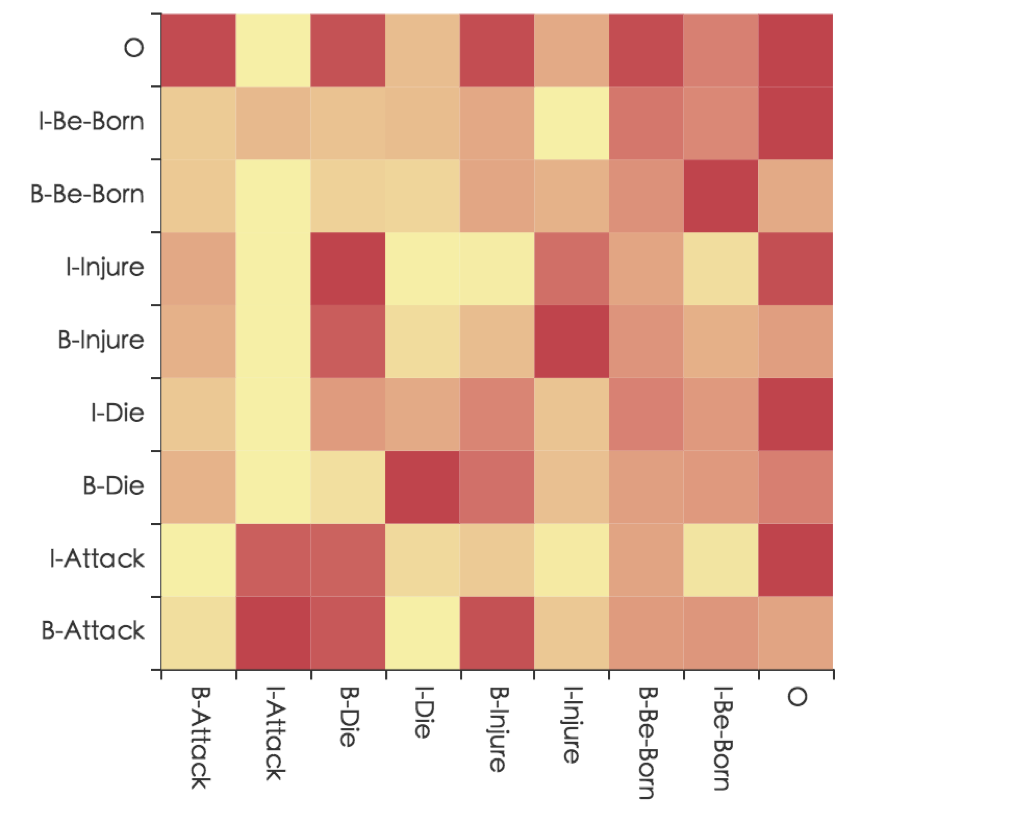
\includegraphics[width=.5\textwidth]{CRF.png}
	\caption{A visualization of a submatrix of transition score in CRF layer. The horizontal axis represents label of current word and the vertical axis represents label of previous word. The darker the color, the higher the score.}
	\label{figure3}
\end{figure}

In Table~\ref{tab:two}, we can see that our character-based convolution BiLSTM-CRF model significantly outperforms other state-of-the-art methods. We list the performance on different types of triggers by C-BiLSTM-CRF and C-BiLSTM model in Table~\ref{tab:three}. Compared with C-BiLSTM models, instead of modeling tagging decisions independently, C-BiLSTM-CRF model takes into account the correlations between labels, which contributes to a 2\% increase of F1 in regular trigger identification, and a 7.7\% increase of F1 in inside-word trigger identification.
We select a subset of labels and generate a heat map in Figure~\ref{figure3} from the transition scores between each label. We find that the better performance of C-BiLSTM-CRF model can be further explained by the following two reasons:
\begin{enumerate}
	\item A CRF layer characterizes the constraints nicely: for a specific event type \texttt{Type}, \texttt{I-Type} can only follow \texttt{B-Type} or \texttt{I-Type}. In other words, if the current label is \texttt{I-Type}, the transition scores for previous labels, except \texttt{B-Type} and \texttt{I-Type}, are invalid and supposed to be very low. For example, as the forth column shows, going from \texttt{B-Die} or \texttt{I-Die} to \texttt{I-Die} is encouraged, while other transitions, like \texttt{B-Attack} to \texttt{I-Die} or \texttt{I-Injure} to \texttt{I-Die} are discouraged.
	\item A CRF layer models the co-occurrences of several event types. For example, an \emph{Attack} event is usually followed by an \emph{Injure} event or a \emph{Die} event. As a result, in the first row, the transition scores of going from \texttt{B-Attack} to \texttt{B-Injure} or \texttt{B-Die} are much higher than other labels start with \texttt{B-}, such as \texttt{B-Be-born}.
\end{enumerate}

Figure~\ref{figure43} shows the whole transition matrix after training. The darkest color grids always appear right below the diagonal, which suggests that for a given label \texttt{B-type}, its most likely following label is \texttt{I-Type}. As we can conclude from Figure~\ref{figure4}, during training, CRF layer gradually learns a score for going from one label to another label and encourages valid paths of labels, while discouraging other invalid or unusual paths.

\begin{figure}
\centering
\subfigure[Initial transition matrix]{\label{figure41} 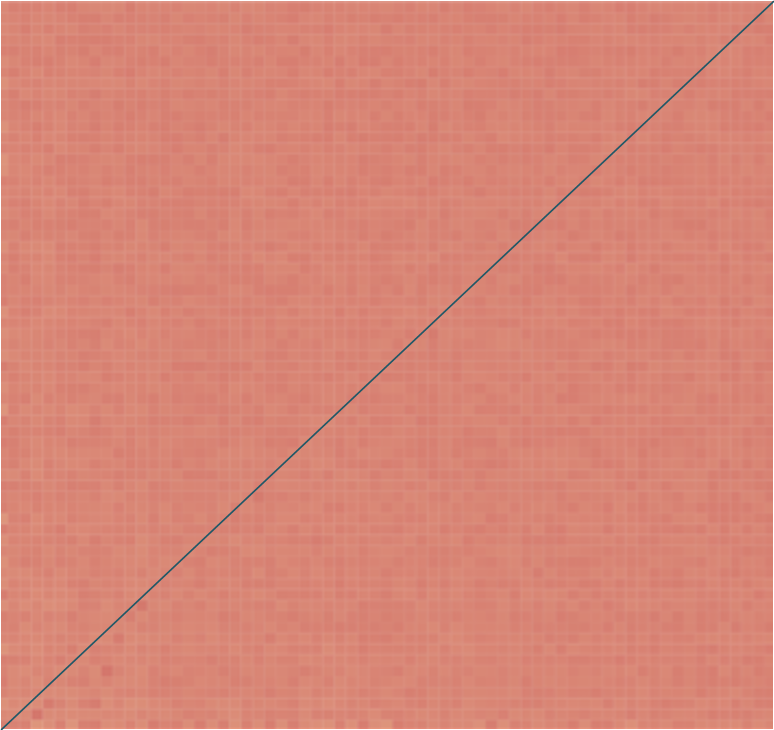
\includegraphics[width=0.32\textwidth]{CRF2}}
\subfigure[Epoch=5]{\label{figure42} 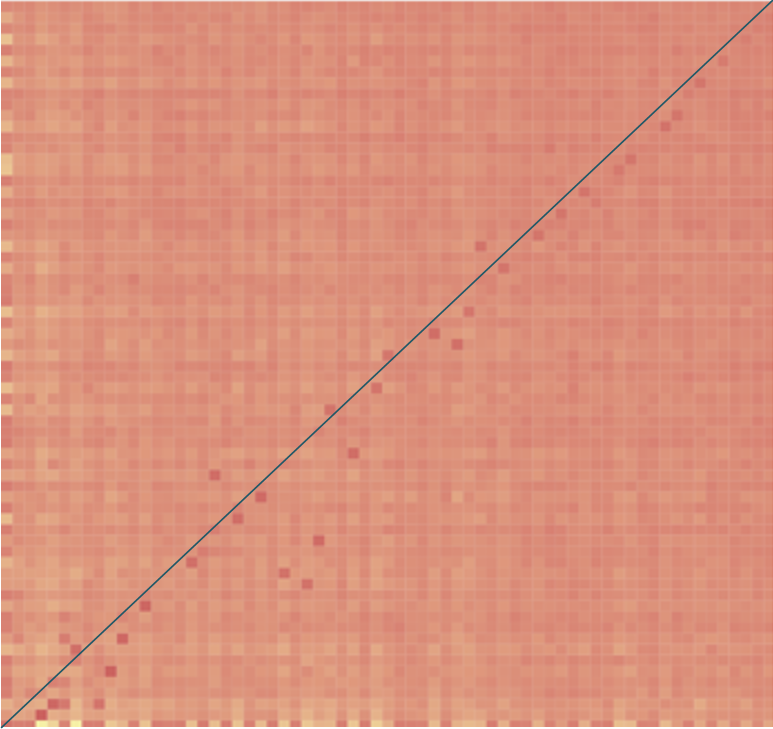
\includegraphics[width=0.32\textwidth]{CRF3}}
\subfigure[Epoch=10]{\label{figure43} 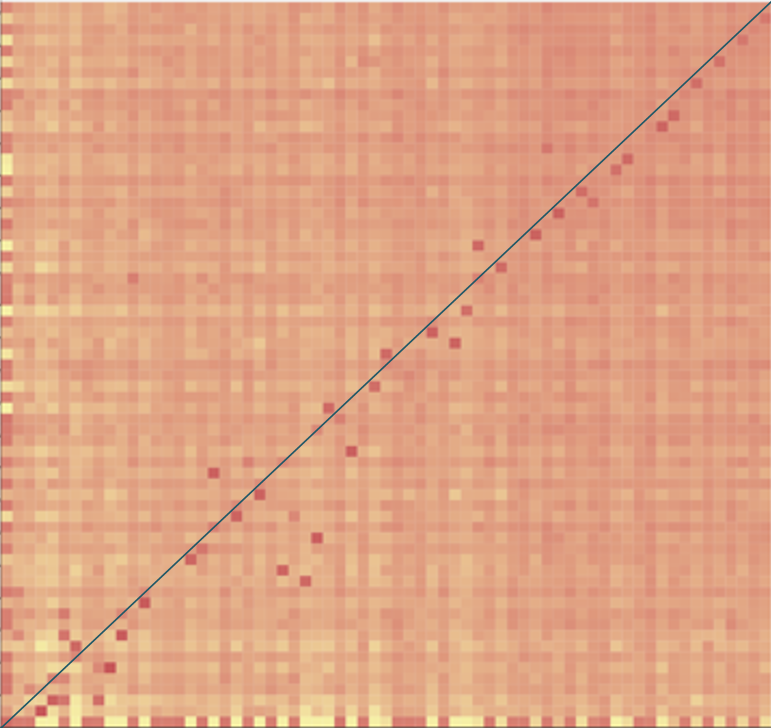
\includegraphics[width=0.32\textwidth]{CRF4}}
\caption{Transition score matrix in CRF layer during training, visualized with heatmaps. Axes have the same meaning as Figure~\ref{figure3}: the horizontal axis represents label of current word while the vertical axis represents label of previous word. Labels in both axes are arranged by their types in the same order as Figure~\ref{figure3}, i.e., \texttt{O, B-type1, I-type1, B-type2, I-type2, B-type3, ...}}
\label{figure4}
\end{figure}
\section{Related Work}\label{related}
Event extraction is one of the challenging tasks in information extraction. Many approaches have been explored from different views, which can be divided into  traditional feature-based methods and neural-network-based methods.

Feature-based methods exploit various feature extraction strategies and evaluate feature contributions for prediction. \citeN{ahn2006stages} models the event extraction task as a pipeline of four classification tasks and applies lexical features (e.g., full word, word lemma, etc.), syntactic features (e.g., dependency trees, SRL structures, etc.), and  features generated from external knowledge resources (e.g., WordNet). Later studies also employ context  sentences and higher level information to characterize global features. For example, \citeN{ji2008refining} utilize global evidence from a cluster of topically-related documents to break down the document boundaries for event extraction. And \citeN{patwardhan2009unified} consider both local context and a wider sentential context around a phrase  to estimate whether a sentence is discussing an event of interest. \citeN{gupta2009predicting} employ cross-event features to extract implicit time information. \citeN{liao2010using} explore document level cross-event information to resolve ambiguities between certain types of events. \citeN{hong2011using} leverage cross-entity inference to predict event mentions.  \citeN{huang2012modeling}  propose a bottom-up approach that initially identifies candidate argument independently and then uses that information to model textual cohesion. More recently, some researchers have tried to improve other aspects of event extractions. As opposed to traditional pipelined approaches, \citeN{li2013joint} attempt to jointly learn all ACE event extraction subtasks using structured perceptron and incorporate global features which explicitly capture the dependencies of multiple triggers and arguments in a transition system.

Recently, neural network models have been employed to achieved competitive performances against traditional models in many NLP tasks. \citeN{chen2015event} propose a convolutional neural network (CNN) to capture lexical-level clues, with a dynamic multi-pooling layer to capture sentence-level features. Recurrent neural network (RNN) is also a popular and effective choice for classification tasks. \citeN{ghaeini2016event} effort to detect triggers that can be either words or phrases by a forward-backward RNN. Nguyen et al. [2016] propose a bidirectional RNN with various memory matrices to jointly learn triggers and arguments, which benefits from the advantages of both joint models and neural network models. \citeN{feng2016language} introduce a language-independent hybrid neural network model that incorporates both bidirectional LSTMs and convolutional neural networks, which yields competitive performances on both English and Chinese event extraction.

Compared to the amount of work on English event extraction, there are a few studies focusing on Chinese event extraction, and most of them are feature-based methods. \citeN{chen2009language} are the first to report the language specific issues in Chinese trigger labeling, and apply various kinds of lexical, syntactic and semantic features to the modularized pipeline system.  One of their simple yet effective strategies is to build an errata table to deal with the inconsistency between word segmentation results and trigger annotations. The table includes the correspondence between words and their frequent labeling results, e.g., the word ``打死'' is often labeled as ``打''$-$\emph{Attack} and ``死''$-$\emph{Die}, and during testing, if the word ``打死''  has been identified as a trigger candidate, we will directly label each character with their specified event types in the errata table, respectively.  However, this strategy is incapable to handle the ``落入法网'' case, where ``落入'' and ``法网'' are usually treated as two words, since the candidate search space is vast. 
 \citeN{li2012employing} also explore language phenomena in Chinese event extraction, and alleviate the word segmentation errors via compositional semantics inside Chinese triggers and discourse consistency between Chinese triggers. The state-of-art feature-based model investigates two extensions to \citeN{li2012employing}, namely joint-learning method and knowledge-rich method. As for the first extension, they divide the original four-step pipeline system into two joint learning tasks where they jointly learn trigger identification and trigger classification, and then jointly learn argument identification and argument classification. In the second extension, they apply six groups of features motivated by deep investigations on the dataset: zero pronoun features and trigger type consistency features  extracted by well-designed rules,  syntactic and semantic features extracted using a Chinese semantic role labeling system, and also help from external linguistic resources, e.g.,  a Chinese synonym dictionary for character-based features. As we can see,  this method heavily relies on elaborate feature templates and external tools or thesauruses, thus may suffers from the errors propagated from other NLP tools.

In this paper, we follow the two-step joint-learning style that alleviates the error propagation problems of traditional pipeline systems, and propose two neural network models to avoid heavy feature engineering and extra resources. Specifically, the CNN component learns lexical features while the bidirectional LSTM component extracts sentence-level features automatically. We further combine a CRF layer to learn sequence labeling preferences to jointly decode the best labels. % \textbf{And these models are flexible that both two subtasks share the similar neural network architectures}.
To further deal with specific issues with respect to Chinese, we,  instead of labeling word by word, we introduce the character-based models to avoid the reliance on carefully designed resources for Chinese event extraction.

\section{Conclusion}\label{conclude}
In this paper, we propose a novel convolution bidirectional LSTM-CRF model on Chinese event extraction task. Our model departs from the inherent characteristic of Chinese language, formulates the event detection task as a sequence labeling fashion, and features both bidirectional LSTM and CNN to capture both sentence-level and lexical features from raw text. Experimental results show that without human-designed features and external resources, our neural network method can achieve state-of-the-art performances on ACE 2005 datasets. In the future, we will explore more global evidences, from both discourse level and cross document level,  to further alleviate the language specific issues, such as the zero pronoun phenomenon in Chinese. Currently, many event extraction methods utilize the type consistency between triggers or arguments as a post-processing step or a set of consistency-check features to prune the extraction results, which should be treated jointly in the extraction models, hopefully in a neural network fashion. And, we will also attempt to model the whole event extraction task  in an end-to-end paradigm to further jointly deal with trigger and argument labeling, avoiding feature engineering or other resources.   


\end{CJK}


% Bibliography
\bibliographystyle{ACM-Reference-Format-Journals}
\bibliography{bibfile}

\medskip

\end{document}
% End of v2-acmsmall-sample.tex (March 2012) - Gerry Murray, ACM
